\section{Background}
We now establish conventions used in this paper, and familiarize the reader with basic concepts for distributed training.


\subsection{Training a ML model}
Different types of models may appear to have different ways of training, but sitting at the center of most models is the common notion of parameters and gradients. Parameters are the goals: they define the ultimate models; gradients are the means: they are derived with respect to parameters, and guide how parameters should be adjusted to minimize the errors (together with a learning rate), usually in an iterative manner, using the technique gradient descent (SGD)~\cite{subgradient,DBLP:journals/corr/Ruder16} (or its variant). 

To illustrate the training process, we use the example of training a deep learning (DL) model, or a deep neural network (DNN), for its popularity. We will continue to explain in the context of DL models throughout this paper for consistency. Modern DL models can have hundreds of \textit{layers} making up multi-megabyte-size \textit{models}. The training process has three phases. In the \textit{forward pass}, a prediction is generated for an input. In the \textit{backward pass}, the prediction is compared with a label to calculate prediction error; then, through \textit{backpropagation}~\cite{backprop}, the gradient for each parameter
is calculated with respect to this error. The model is then \textit{updated} using these gradients, often using a variant of the SGD algorithm. Each Computation is often done on GPUs or other accelerators suited to regular data-parallel operations, processing a batch of samples at once (\textit{minibatching}).
%Multiple examples are processed in each GPU simultaneously in a single \emph{minibatch} which typically contains tens to hundreds of samples. 
%Each GPU processes multiple examples simultaneously in a \emph{minibatch} which typically contains tens to hundreds of samples. 

\begin{figure}[t!]
	\centering
	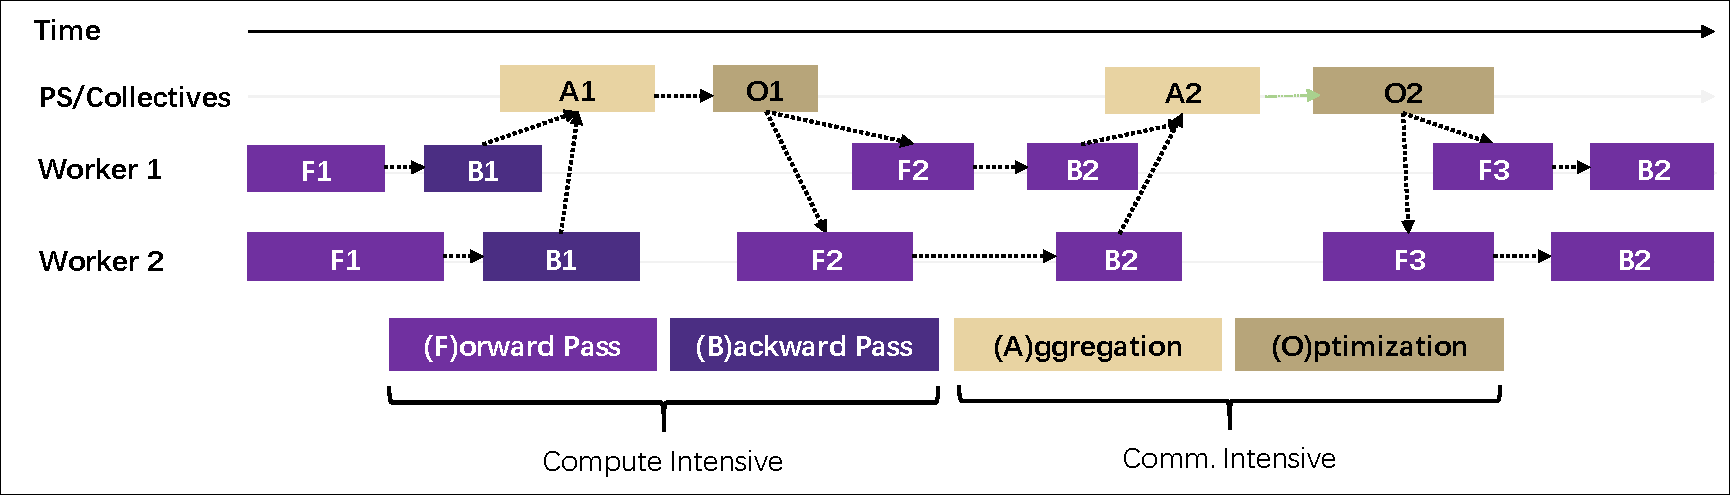
\includegraphics[width=.6\linewidth, trim=2 3 3 3,clip]{Figures/distributedtraining.pdf}
	\caption{A few iterations of distributed training pipeline of neural networks.}
	\label{fig:distributedtraining}
\end{figure}

\subsection{Distributed Training}
Broadly speaking, there are two extremes in terms of paradigms in distributed training: \textit{data} parallelism and \textit{model} parallelism, and many hybrid systems strike a balance between these two.

In data parallelism, training data is pre-partitioned to each individual workers, and each worker sees only a partition of the data. In model parallelism, instead of partitioning training data, the model itself is being partitioned.% This is handy because the multi-layer of modern DL models and well-defined dependencies make it simple to partition the model to different nodes. A piece of data then follows through the entire system, as if in the single node training case, except that it crosses node boundaries.

This paper mainly focuses on data parallelism, as it is the default choice in many frameworks and practices. The distributed training process (Figure~\ref{fig:distributedtraining}) using data parallelism is different in a few ways from training within a single node.
%First, a mean gradient is calculated for each minibatch in each GPU. %
First, a mean gradient is calculated across all minibatches in each machine. Then, the mean of the gradients from each machine is calculated. Finally, the model is updated based on that mean, new parameters are broadcast to each machine and GPU, and the next batch is trained. This paper focuses on optimizing calculation of both the mean gradient across machines and the subsequent model update (or \textit{parameter exchange}). Note that gradient aggregation and model optimization are both element-wise operations.

%n the second, each worker also stores a shard or replica of the global model; model updates are done through collective communication operations involving all machines.

The process described here is \textit{synchronous training}, where all machines and GPUs execute a new minibatch simultaneously and update the model based on the gradients in the current iteration. It is also possible to train asynchronously~\cite{tensorflow,revisitSGD,GeePS,recht2011hogwild,projectAdam,googleDNN}, sacrificing reproducibility for a potential throughput increase. %updating the model with the gradient from each GPU's minibatch with little or no synchronization among machines; this can improve throughput in some situations but may limit repeatability and debuggability. 
We focus on synchronous training due to its simplicity and commonality in industry, but our techniques can also benefit asynchronous training.

\begin{figure}[t!]
	\centering
	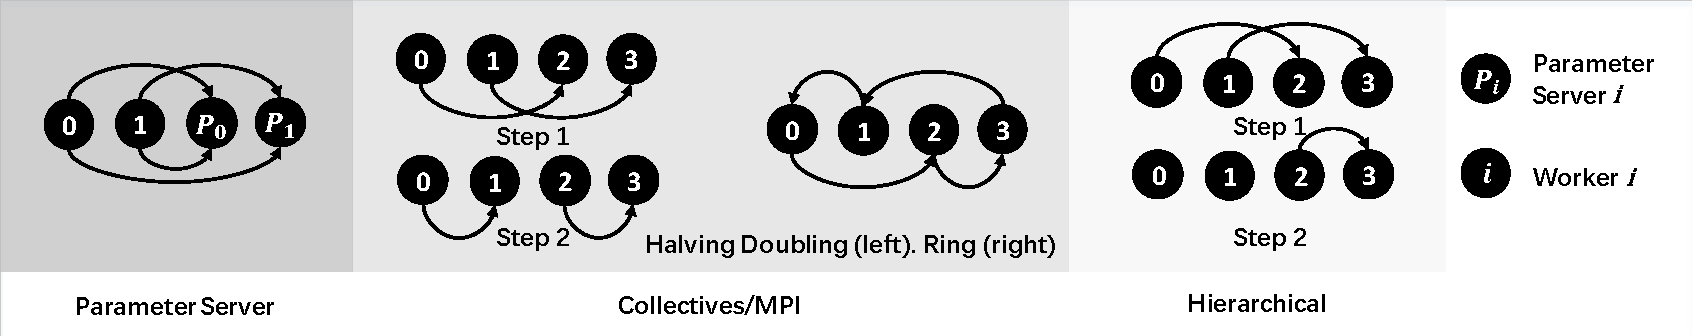
\includegraphics[width=\linewidth, trim=2 3 3 3,clip]{Figures/aggregationapproaches.pdf}
	\caption{Aggregation is commonly done with one of the three prevailing paradigms, parameter server, collectives all-reduce, and hierarchical aggregation in practice.}
	\label{fig:aggregationapproaches}
\end{figure}


\begin{figure}[t!]
	\centering
	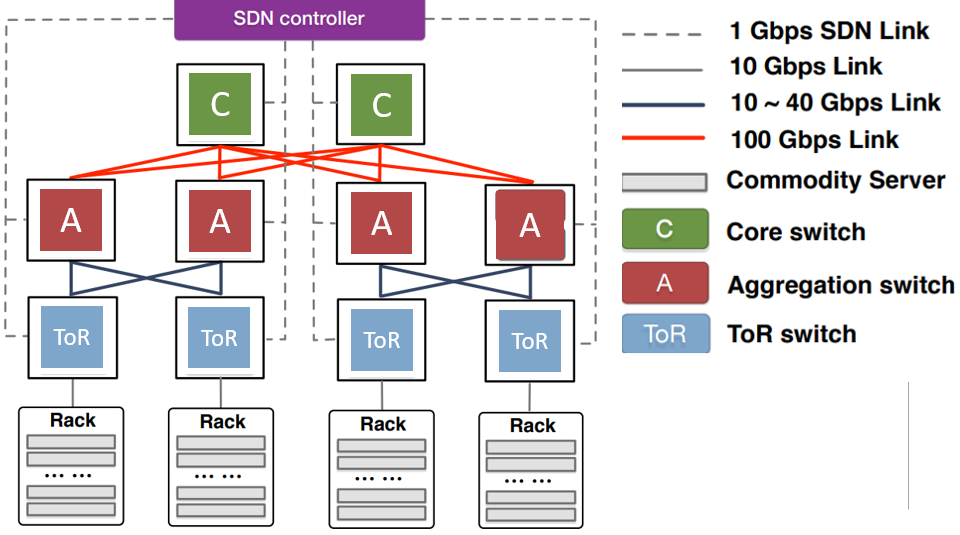
\includegraphics[width=.6\linewidth, trim=2 3 3 3,clip]{Figures/dc.png}
	\caption{Overview of a typical datacenter network topology.}
	\label{fig:dc}
\end{figure}


\subsection{Datacenter Network Topology}
\label{sec:datacenternetwork}
A typical datacenter network has a hierarchical, multi-tiered topology~\cite{Mysore2009PortLandAS,VL2,Roy2015InsideTS,incbricks} (Figure~\ref{fig:dc}). Machines are grouped into \textit{racks}, each connecting to a top-of-rack \textit{(ToR)} switch. ToR switches are connected to multiple upper level devices. This setup poses challenges for existing training systems: in this setting, the communication performance of two end-hosts is affected by where they reside: they enjoy full link bisection bandwidth within a rack, because link capacity is not shared at the rack-level, but if they are on different racks, the communication performance depends on link congestion and oversubscription ratio~\cite{Bilal2012ACS}. In this paper, we use \textit{locality} to refer to the cause of variation in communication performance, which includes: (1) physical topology: the location of the nodes and (2) dynamic network load. Efficient communication requires carefully architecting software to tap into both aspects~\cite{eyeQ, 27Octobe15:online}: solutions that ignore physical topology are subject to long-term communication imbalances, and those that ignore dynamic network load suffer from short-term inefficiencies.

\subsection{Distributed Training is Here to Stay}
Faster and more powerful accelerators (most notably TPUs~\cite{Jouppi:2017:IPA:3079856.3080246} and Nvidia DGX~\cite{AIResear61:online}) open up the possibility of training in a single device. It all of sudden seems plausible to build a ``supercomputer'' for training, which completely eliminates the need for costly communication. 

Unfortunately, building a training supercomputer does not avoid the problem of insufficient compute resources, but only delays it, for at least two reasons: from a historic perspective, it never happens that there is a surplus in the compute power when it comes to new models, as shown in Table~\ref{table:trend}: scientists can always find models whose complexities are well beyond reach of a single device, which frequently ended up being trained in a distributed fashion: i.e., the use of a single device (e.g. DGX) is not because that single device covers all the need, but rather the lack of additional devices; from an architecture perspective, compute density cannot scale forever as many hard limits are imposed on the number of transistors to fit on a fixed area, including physical effects and cooling constraints. When near these limits, it gets prohibitively difficult to build faster chips within a confined area. 

On the other hand, any training that spans device boundary, not necessarily machine boundary, can be classified as distributed training, and the communication medium need not be limited to conventional network media, but can also include device buses. With this broad view, distributed training is inherent in deep learning. In fact, many have already started looking into optimization of inter-device communication within a single machine~\cite{wang2019blink}. %at each hierarchy (GPU vs PCI-E, Node vs Ethernet), we can observe large gap between the bandwidth of communication and compute. 

\subsection{Gradient Aggregation: Common Practices}
In a loose taxonomy, collecting gradients for aggregation (known as parameter exchange) is commonly done with one of the following paradigms (Figure~\ref{fig:aggregationapproaches}).


\begin{figure}[t!]
	\centering
	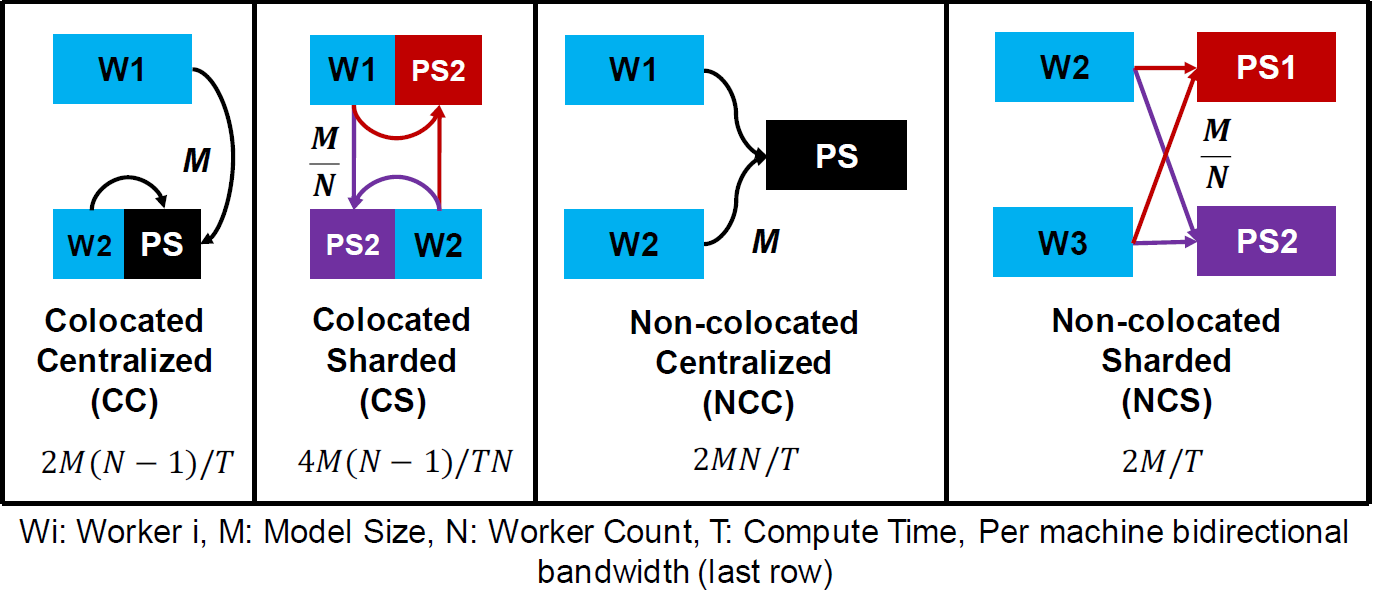
\includegraphics[width=.7\linewidth, trim=2 3 3 3,clip]{Figures/pssetups.PNG}
	\caption{Aggregation is commonly done with one of the three prevailing paradigms, parameter server, collectives all-reduce, and hierarchical aggregation in practice.}
	\label{fig:pssetups}
\end{figure}

\noindent\textbf{Parameter Servers (PS)}~\cite{ps0,ps1,ps2,ps3, phubsocc, phubsysml, poseidon,cui2016geeps}. %Nodes are assigned the role of \textit{workers} or \textit{servers}. 
PSs are key-value stores, where keys and values represent the model's layer IDs and parameters. PSs are well-suited for training at a small scale. PSs can be centralized or sharded. In each iteration, all workers update the model stored in PSs with their locally-produced gradients. PS configurations primarily differ along two axes: colocated (C) versus non-colocated (NC), and centralized (C) versus sharded (S). %In a colocated setting, a PS process can run with worker processes in the same machine. In a non-colocated setting, a machine is dedicated to a worker or a PS process.  
A PS setup is colocated if a worker and a server process share the same physical machine. A PS setup is centralized if a single PS process handles all keys; and a sharded setup load-balances keys across multiple PS processes.
%A centralized PS stores the entire model, whereas each sharded PS stores only a partition of the keys in the entire key space. The size of each partition is usually balanced by the available hardware resources. 
During synchronization, each worker sends and receives model updates from each PS process. Figure \ref{fig:pssetups} illustrates the four combinations of choices from these two axes: Colocated Centralized (CC), Colocated Sharded (CS), Non-colocated Centralized (NC) and Non-colocated Sharded (NCS).

In general, sharded PSs scale better at higher hardware costs. Colocated PSs reduce total data movement on the network by $\frac{1}{N}$ with $N$ workers participating: the update for the partition of the model assigned to a colocated PS need not go through the network. While many frameworks default to CS configurations~\cite{MXNetont0:online, Distribu25:online}, in a colocated setup the PS process interferes with the training process, because both are contending for network and processing resources. Specifically, compared to NC PSs, \textit{each network interface must process roughly 2x the network traffic, because both the colocated worker and PS processes must send and receive model updates from remote hosts}, creating a major bottleneck in network-bound distributed training. 

\begin{figure}[t!]
	\centering
	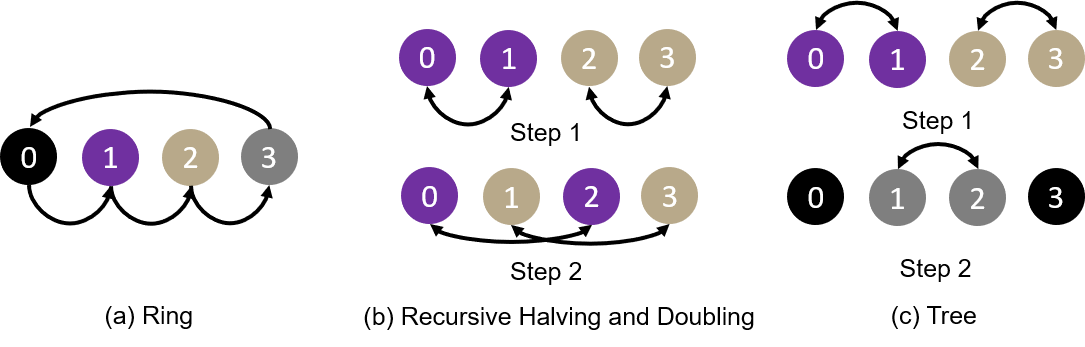
\includegraphics[width=.6\linewidth]{Figures/collectivesAlgorithms.png}
	\caption{Rounds of communications (color-coded) in various popular \collectives algorithms with 4 nodes.}
	\label{fig:collectivesAlgorithm}
\end{figure}

\noindent\textbf{Collective AllReduce (CA)}~\cite{Sack:2011:SCM:2522220,Thakur:2005:OCC:2747766.2747771,collectivesOptimization,blum2000architectures,bala1995ccl}. Popular in the context of MPI, CAs are widely used in larger-scale training. All nodes in CA participate in the communication, usually running symmetric tasks. The end goal of CA is that all nodes have a globally-reduced copy of the data. Widely used CA in training deep learning models include halving-doubling~\cite{ImageNetIn1Hour}, ring and double binary tree~\cite{Operatio73:online, Sergeev2018HorovodFA}. We characterize some of the popular \cmpi here.

\noindent\textit{Ring}~\cite{patarasuk2009bandwidth}. As shown in Figure~\ref{fig:collectivesAlgorithm}(a), ring algorithm works by connecting nodes to form a virtual ring. Data is then passed along the ring sequentially. Ring algorithm requires $O(N)$ steps to complete, sending $O(NS)$ amount of data.

\noindent\textit{Halving Doubling}~\cite{Thakur:2005:OCC:2747766.2747771}. As shown in Figure~\ref{fig:collectivesAlgorithm}(b), halving doubling works by recursively doubling the distance (in terms of rank ID) while halving the total amount of data sent in each round, requiring $O(log_{2}{N})$ steps to finish while also sending $O(NS)$ amount of data on wire.

\noindent\textit{Tree}. Tree algorithms are versatile, in a simple form a single tree is built where data is transferred from leaves to the root and vice-versa~\cite{firecaffe}; in a more optimized setting, a pair of complementary binary trees are built to fully utilize the full bisection bandwidth~\cite{dbt}, each sending and receiving $S/2$. For binary tree \collectives algorithms, $O(log_2N)$ rounds of communication are required, also sending $O(NS)$ bytes on wire. 

\noindent\textit{BCube}~\cite{glooalgo70:online}. BCube is very similar to halving doubling from a structural perspective, in the sense that nodes are organized into group of $B$ peers. BCube operates in $O(log_BN)$ rounds, and each node in each round would peer with an unique node in another $B-1$ groups. Each node communicates $\frac{S}{B^i}$ amount of data in round $i$. BCube achieving a total bytes on wire of $O(\sum_{i=0}^{log_BN-1}\frac{S}{B^{i+1}})$.

CAs and PSs are not mutually exclusive. Using one does not exclude the use of other. For example, ~\cite{10.1145/3302424.3303957} dynamically chooses CA or PS based on sparsity of a given key.

Gradient aggregation can be \textit{flat} (e.g., use of PSes and CAs are generally flat) or \textit{hierarchical} (Hierarchical Aggregation, HA), which refers to the generic technique of aggregating data in multiple steps, from local to global. Exemplar usage of HA in the distributed training context include~\cite{firecaffe,choblueconnect,Geng:2018:HHP:3229543.3229544,sysmlblueconnect}, though in the context of proprietary networks. HA is highly flexible and supports mix and matching of multiple aggregation paradigms~\cite{topoawarempi, cool}. Hierarchical schemes are essential in enabling large-scale training. 

This paper mainly focuses on the discussion of building efficient PSs, but most of the techniques still apply to accelerating CAs as well. We dedicate sections related to \cmpi to CAs. 

\subsection{More Efficient Distributed Training: Prior Arts}
Approaches to accelerating distributed training can be classified into one of the broad categories in the current literature.

\noindent\textbf{Synchronize less often}. One way to achieve a lower synchronization frequency is to oversubscribe GPUs. This can be done by using a very large batch size, fully utilizing GPU memories, making GPU compute the bottleneck~\cite{Nowanyon13:online, ImageNetIn1Hour, sridharan2018scaleout, jia2018highly, you2019large,you2017large}. Large batch sizes reduce communication frequency. However, this eliminates the potential of achieving a larger speedup with fast communication. For example, with ResNet-50, ~\cite{Shen2018NexusA} shows only 10 samples are needed to fully utilize a recent GPU. This means the computation of large batches can be further spread to more GPUs, and additional throughput is attainable provided that communication overhead is low. Further, large batch optimization is also not universally available (requiring GPUs with large memory) and may be subject to worse generalization~\cite{keskar2016large}.

Orthogonal to large batch optimization, another line of work target at less synchronization. They tune the consistency model of distributed training, with relaxed consistency~\cite{DBLP:journals/corr/DaiKWHGX14,SSP,BSP,Wei:2015:MCC:2806777.2806778,Litz,xie2018orpheus,wang2018adaptive}. Generally, these relaxed consistency models do not mandate a strict barrier for synchronization at iteration boundary, and instead, they allow staleness in the model and a potential different view of model from each worker, removing the synchronization overhead from the critical path. However, these methods suffer from difficulty in reproducing the models. 

\noindent\textbf{Send less data}. Sending less data accelerates distributed training in a bandwidth-bound environment, and can be achieved through (1) lossless compression~\cite{burtscher2009fpc}; (2) lossy compression, removing redundancy in the SGD algorithm~\cite{lin2017deep}; (3) quantizing update gradients to low bit representations and locally apply residual errors~\cite{cntk1bt, lim20183lc} and (4) decomposing large update matrices~\cite{projectAdam,poseidon,xie2015distributed} and reconstructing at destination. These methods either trade more computation for less communication, or risk affecting the final convergence accuracy of the model, and both of which may turn out \textit{increasing} the total wall clock time required to reach the target accuracy.

\noindent\textbf{Build faster clusters}. Another series of work involves building specialized hardware clusters for distributed training with quick interconnects to tackle communication bottlenecks~\cite{DBLP:journals/corr/abs-1711-00489, You:2018:ITM:3225058.3225069, DBLP:journals/corr/abs-1711-04325,jia2018highly,DBLP:journals/corr/abs-1811-05233,sun2019optimizing, ImageNetIn1Hour, firecaffe}. While the results have been encouraging, these approaches demand steep investments and are not available to everyone.

\noindent\textbf{Hide communication latency}. Most modern frameworks encode the model being trained as a dataflow graph. An operator is executed as soon as its dependencies are resolved, and this allows overlapping of communication and computation during the backpropagation stage of distributed training. Some work even attempt to re-prioritize sending of first layers over later layers to deal with this priority inversion problem. Notable applications of this idea include~\cite{hashemi2018tictac, prioritybased, poseidon, 10.1145/3341301.3359642}. However, communication latency hiding has severe limits: faster computation device leaves smaller room; many model training is in fact bandwidth bound, and hiding latency only has limited impact on the total training time.

\noindent\textbf{Use finer-grained parallelism}. This can be done by blending in higher compute hardware utilization of data parallelism and lower communication cost of model parallelism to form pipelined parallelism~\cite{harlap2018pipedream}. This can also be done by allowing a flexible combination of slicing along arbitrary dimensions of S(ample)O(perator)A(ttribute)P(arameter), enabling more execution possibilities and effectively enlarging the action space. More efficient schedule can then be determined by intelligently searching through the enlarged space by taking communication cost into account~\cite{jia2018beyond}. However, these methods have the limit of needing to research as soon as the underlying hardware environment, or the models being trained change.

\noindent\textbf{Accelerate at network level}. The emergence of programmable network devices open up the opportunity to accelerate distributed training at the core of network, allowing gradient aggregation in the network devices, resulting in lower parameter exchange latency and lower bandwidth requirement (e.g. broadcast of aggregated model can be efficiently done with a network switch~\cite{sapio2019scaling,luomotivating}). Current programmable devices are not without limits, enforcing hard constraints on compute and memory.

\noindent\textbf{Improving cluster-level efficiency}. A series of work ~\cite{222611,Shen2018NexusA} target at an orthogonal goal, and instead of optimizing for each individual task, they aim to achieve an average high utilization of compute resources in a cluster, by time-sharing (preemption) and better placement.


